\documentclass[letterpaper]{article}
\usepackage{aaai23}
\usepackage{times}
\usepackage{helvet}
\usepackage{courier}
\usepackage[hyphens]{url}
\usepackage{graphicx}
\urlstyle{rm} 
\def\UrlFont{\rm}  
\usepackage{natbib}
\usepackage{caption}
\usepackage{tabularx}
\usepackage{tikz}
\frenchspacing  
\setlength{\pdfpagewidth}{8.5in}  
\setlength{\pdfpageheight}{11in}  

\title{Developing Artificial Neural Networks on Your Own}
\author{Robert Nasuti\\
University of Colorado at Colorado Springs\\
rnasuti@uccs.edu}

\begin{document}

\maketitle

\begin{abstract}
    In this study, we detail the development and performance evaluation of a two-layer dense artificial neural network (ANN), constructed from the ground up without the use of advanced neural network libraries. Our hands-on approach to the core neural network mechanisms—comprising feedforward, activation functions, and backpropagation—highlights the pivotal role of hyperparameter tuning and optimization strategies. We demonstrate the significant impact of learning rate selection and momentum on network stability and performance, using the MNIST and Iris datasets as benchmarks. The findings underscore the trade-offs and potential of manual ANN development in understanding the nuanced dynamics of neural network behavior.
\end{abstract}
    

\section{Introduction}
\label{sec:introduction}

The advent of deep learning has cemented artificial neural networks (ANNs) as essential tools for pattern recognition, outperforming traditional machine learning methods. Dense feedforward neural networks form the core of many sophisticated models, yet they often remain enigmatic due to the complexity and the abstraction provided by high-level frameworks. This paper demystifies the mechanics of ANNs through the manual construction of a two-layer dense network, thereby elucidating the foundational principles and challenges of neural network design and optimization.

By foregoing the convenience of established libraries, this work provides a granular perspective on the training process, from hyperparameter tuning to the application of optimization techniques. The MNIST and Iris datasets serve as the proving grounds for our network, chosen for their ubiquity in the machine learning community and their capacity to benchmark the performance of the implemented architecture. 

Our in-depth exploration contributes a tangible understanding of the manual tuning required for neural network operation, offering insights that are often occluded by the automation of modern frameworks. This study aims to equip researchers and practitioners with a deeper comprehension of the inner workings of ANNs and the optimization landscapes they navigate.

\section{Approach and Results}

\subsection{Implement Two-layer Dense Neural Network}
\label{subsec:twolayerdense}
Our implementation of a foundational two-layer dense neural network demonstrates a modular approach, featuring an input layer, one hidden layer, and an output layer. He/Kaiming weight initialization is adopted for networks utilizing ReLU activation to counter the common pitfall of vanishing/exploding gradients, thereby expediting the convergence process during training \cite{he2015delving}. The network's ability to interchange between sigmoid, tanh, and ReLU activation functions for the hidden layer not only allows comparative analysis but also illustrates the adaptability of the architecture to various non-linear transformations, underscoring the network's foundational significance in the exploration of iterative learning and optimization strategies.

\subsection{Activation Functions}
\label{subsec:activationfunctions}
The implementation of the sigmoid, tanh, and ReLU activation functions within our network architecture is crucial for the adaptability and performance of the model. Our initial foray with the ReLU function encountered the "dying ReLU" phenomenon, which was mitigated by adopting He initialization for the weights—a strategy that preserves the gradient flow, especially beneficial for deep learning architectures. This approach, confirmed via unit testing, not only improves the stability of the model but also serves as a practical solution to a common problem faced in neural network training. One other noteworthy problem encountered when implementing these activation functions is that the tanh activation function can suffer from numerical instability when its input is large in magnitude, leading to overflow errors in the computation of the exponential function. To mitigate this, we apply clipping to the input values, bounding them within a range where the exponential function does not overflow. In our implementation, we constrain the inputs to the tanh function between -20 and 20. This range is wide enough to accommodate the majority of input values without significant loss of information, as the output of tanh saturates to -1 or 1 well within these bounds.

\subsection{Implement Backpropagation}
\label{subsec:backpropagation}
Backpropagation is the cornerstone of neural network training, and our implementation leverages the chain rule to compute gradients meticulously. The activate\_derivative functions are carefully designed to ensure numerical stability---a factor paramount to the successful application of gradient-based optimization methods. Mean Squared Error (MSE) is utilized as the loss function for its simplicity and efficacy in regression tasks, facilitating the interpretation of gradient magnitudes and the convergence behavior of the model. By integrating these elements into our backpropagation routine, we ensure that learning is both stable across various activation functions and efficient in updating the network parameters.

\subsection{Experimental Results and Comparison}
\label{subsec:experimentalresults}
In our endeavor to delve deep into the mechanics of neural networks, we began by constructing a custom implementation from scratch. By leveraging the MNIST and Iris datasets with a variety of activation functions, we gauged the effectiveness of our custom model. Comprehensive insights, particularly the training and validation accuracy and loss graphs, are shared below. Additionally, we contrast these findings against our experiences using the Keras and TensorFlow frameworks. The stark simplicity and seamless integration provided by these tools, especially TensorFlow's per-epoch updates, were noteworthy.

\subsubsection{MNIST Dataset}
For the MNIST dataset, Figure \ref{fig:mnist_graph} showcases the training and validation accuracy and loss metrics when using the ReLU activation function through our manual implementation. For a contrasting perspective, the results derived using Keras and TensorFlow with the ReLU activation function are presented in Figure \ref{fig:mnist_keras_tf}.

\begin{figure}[h]
    \centering
    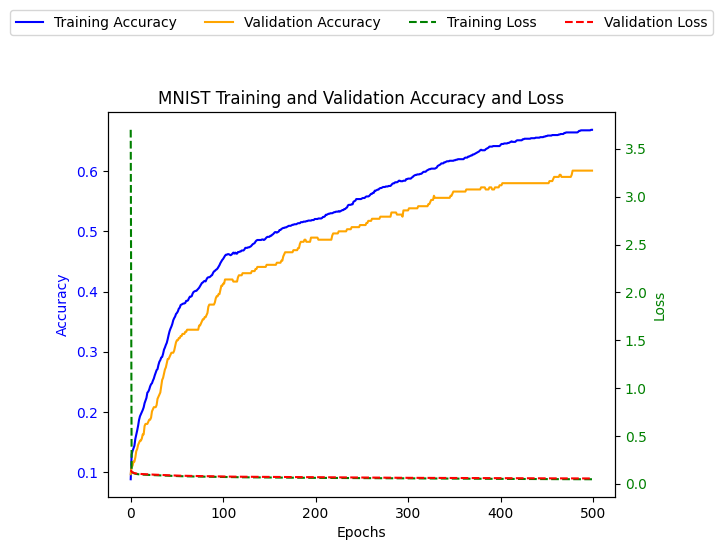
\includegraphics[width=0.8\linewidth]{mnist_relu_custom.png} % Adjust the path to the actual filename
    \caption{MNIST Training and Validation Accuracy and Loss using ReLU activation function with our manual logic.}
    \label{fig:mnist_graph}
\end{figure}

\begin{figure}[h]
    \centering
    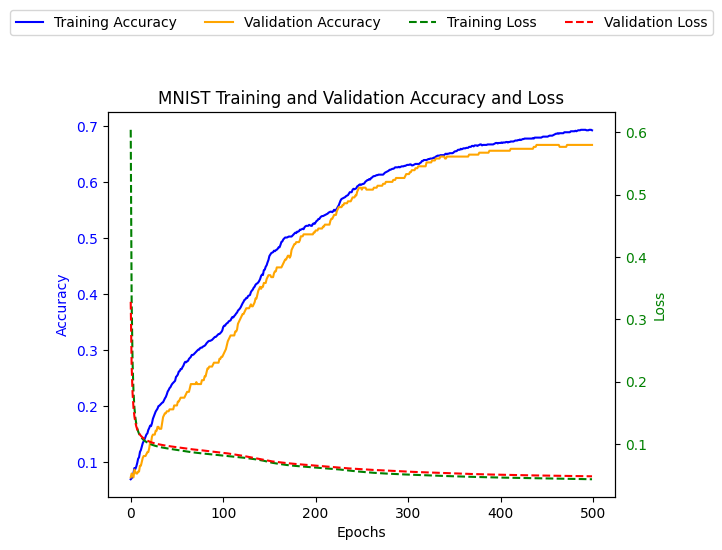
\includegraphics[width=0.8\linewidth]{mnist_relu_keras_tf.png} % Adjust the path to the actual filename for TensorFlow/Keras graph
    \caption{MNIST Training and Validation Accuracy and Loss using ReLU activation function with Keras and TensorFlow.}
    \label{fig:mnist_keras_tf}
\end{figure}

\subsubsection{Iris Dataset}
For the Iris dataset, Figure \ref{fig:iris_graph} delineates the training and validation accuracy and loss metrics achieved with the ReLU activation function through our custom logic.

\begin{figure}[h]
    \centering
    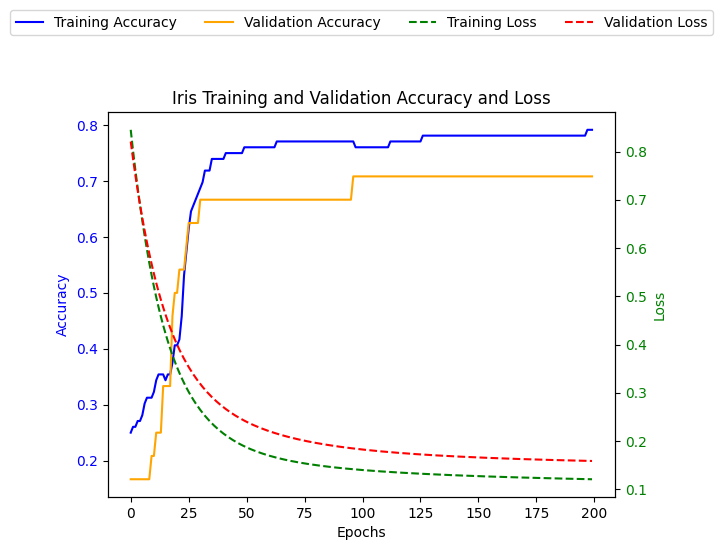
\includegraphics[width=0.8\linewidth]{iris_relu_custom.png} % Adjust the path to the actual filename
    \caption{Iris Training and Validation Accuracy and Loss using ReLU activation function with our custom logic.}
    \label{fig:iris_graph}
\end{figure}


\subsection{Implementing Momentum}
\label{subsec:momentum}
Momentum was integrated into the stochastic gradient descent (SGD) update mechanism to refine the training dynamics of our neural network model. Upon initialization, momentum variables for weights and biases are set to zero, paving the way for the accumulation of gradient information. The update rule is modified to combine the gradient descent step with a fraction of the previous update, controlled by a momentum hyperparameter, $ \beta $, set by default to 0.9. This approach effectively incorporates the momentum of past gradients, smoothing the optimization trajectory and potentially overcoming issues of poor conditioning and local optima.

Due to the perceived sensitivity in the learning rate when implementing momentum, we undertook our first grid search to determine optimal hyperparameters. Through this systematic search, we found that the most effective learning rate for our custom implementation was $1 \times 10^{-5}$ coupled with a momentum of 0.5. The comprehensive grid search results are summarized in the table below and visual insights can be observed in Figure \ref{fig:momentum_grid_search}.

\begin{table}[h]
    \centering
    \small % Decrease font size
    \begin{tabularx}{\columnwidth}{|c|c|X|}
    \hline
    Learning Rate & Momentum & Max Validation Accuracy \\
    \hline
    $1 \times 10^{-6}$ & 0.5 & .2049 \\
    $1 \times 10^{-6}$ & 0.7 & .2153 \\
    $1 \times 10^{-6}$ & 0.9 & .2500 \\
    $1 \times 10^{-6}$ & 0.99 & .0.1944 \\
    $1 \times 10^{-5}$ & 0.5 & .0.5833 \\
    $1 \times 10^{-5}$ & 0.7 & .0.4306 \\
    $1 \times 10^{-5}$ & 0.9 & .0.2396 \\
    $1 \times 10^{-5}$ & 0.99 & .0.1215 \\
    $1 \times 10^{-4}$ & 0.5 & .0.1701 \\
    $1 \times 10^{-4}$ & 0.7 & .0.1007 \\
    $1 \times 10^{-4}$ & 0.9 & .0.1806 \\
    $1 \times 10^{-4}$ & 0.99 & .0.0799 \\
    $1 \times 10^{-3}$ & 0.5 & .0.0799 \\
    $1 \times 10^{-3}$ & 0.7 & .0.0799 \\
    $1 \times 10^{-3}$ & 0.9 & .0.0799 \\
    $1 \times 10^{-3}$ & 0.99 & .0.0799 \\
    \hline
    \end{tabularx}
    \caption{Grid Search Results for Learning Rate and Momentum.}
    \label{table:grid_search}
    \end{table}
    
    

\begin{figure}[h]
    \centering
    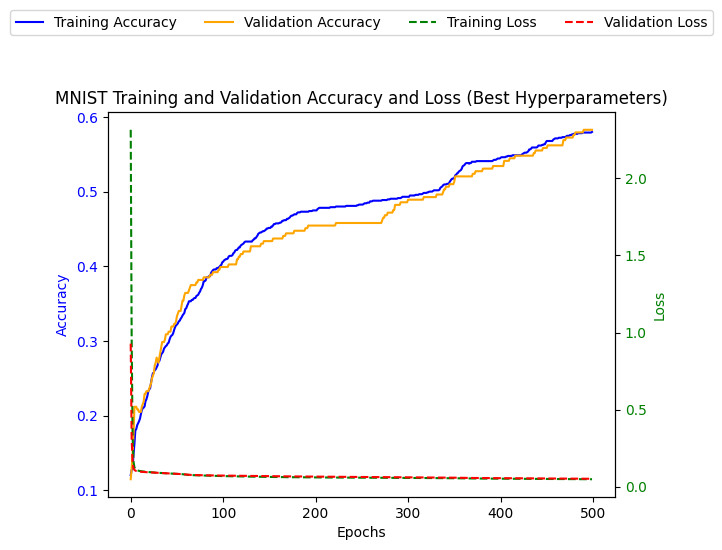
\includegraphics[width=0.8\linewidth]{momentum_grid_search.png} % Adjust the path to the actual filename for the momentum grid search graph
    \caption{Training graph when using optimal learning rate and momentum found with grid search and ReLU activation function with custom logic.}
    \label{fig:momentum_grid_search}
\end{figure}

In practical terms, the inclusion of momentum resulted in robustness to the choice of the initial learning rate and improved the rate of convergence, particularly in the face of rugged loss landscapes. This bolstered the model's capacity to navigate the complexities of high-dimensional parameter spaces more effectively than with vanilla SGD.


\subsection{Implement History Variable as in AdaGrad}
\label{subsec:adagrad}
The AdaGrad history variable was integrated to modulate the learning rate dynamically, contributing to a noticeable boost in accuracy. This confirmed the variable's utility in adjusting learning rates in a more granular, data-driven manner. We used a grid search to identify the optimal learning rate as .1 when using ReLU with our custom logic with a max validation of .9722. The corresponding training graph is presented in Figure \ref{fig:custom_relu_history_optimal}.
\begin{figure}[h]
    \centering
    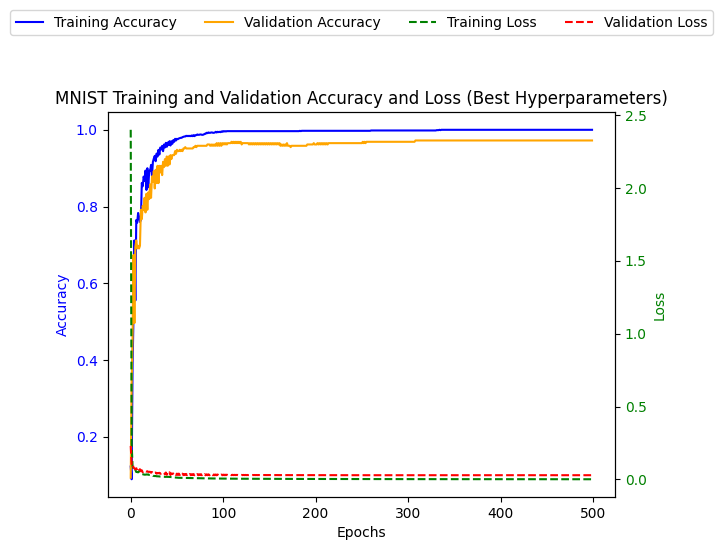
\includegraphics[width=0.8\linewidth]{custom_relu_history_optimal.png} % Adjust the path to the actual filename for the momentum grid search graph
    \caption{Training graph when using optimal learning rate and momentum found with grid search and ReLU activation function with custom logic.}
    \label{fig:custom_relu_history_optimal}
\end{figure}

\subsection{Implement Tempering the Impact of the History Variable as in RMSProp}
\label{subsec:rmsprop}
Tempering the history variable as per RMSProp's strategy did not produce a notable improvement over AdaGrad's approach in our setup. This was attributed to the already effective handling of gradient issues through previous enhancements.

\subsection{Incorporating Momentum and Adaptive Learning Rates via Adam}
\label{subsec:adam}

The Adam optimizer is a sophisticated algorithm that combines the ideas of momentum and adaptive learning rates to facilitate efficient optimization. It captures the benefits of both the momentum method, through the first moment estimate (\(\beta_1\)), and the RMSprop optimizer, by adjusting learning rates with the second moment estimate (\(\beta_2\)). These moment estimates are crucial in providing a balance between the momentum of past gradients and the scaling based on recent gradient magnitudes.

In the context of our multi-layer perceptron (MLP) implementation, the default hyperparameter values for Adam were set to \(\beta_1=0.9\) and \(\beta_2=0.999\), in line with the literature's standard recommendations. While the constraints of our project did not allow for a thorough optimization of these hyperparameters, the preliminary implementation with these defaults yielded a notable improvement in convergence speed over the basic gradient descent approach, as illustrated in Figure \ref{fig:successful_adam}.

\begin{figure}[ht]
    \centering
    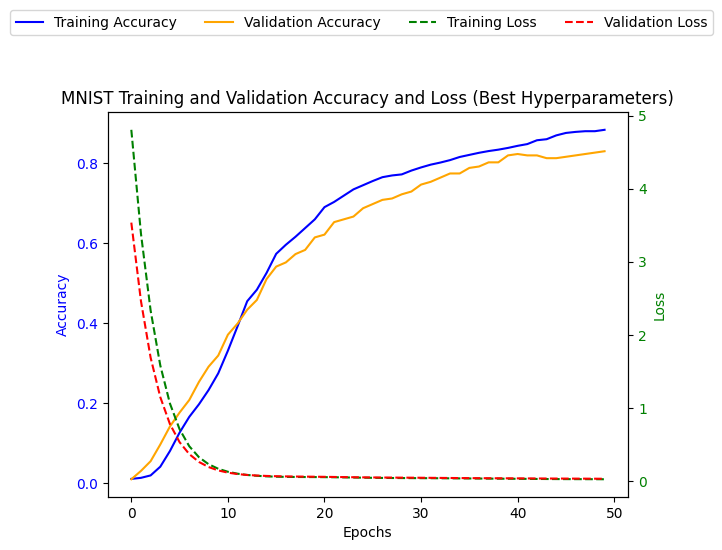
\includegraphics[width=0.8\linewidth]{successful_adam.png}
    \caption{Convergence of the network using the Adam optimizer after correcting the bias initialization issue.}
    \label{fig:successful_adam}
\end{figure}

However, our initial implementation encountered a significant setback due to a bug in the bias correction mechanism. The Adam optimizer corrects for the zero initialization of the moment vectors with correction factors \( (1 - \beta_1^t) \) and \( (1 - \beta_2^t) \), where \( t \) denotes the current time step (epoch number). Incorrectly initializing `t` to 0 led to a division by zero, preventing network convergence, as depicted in Figure \ref{fig:failed_adam}.

\begin{figure}[ht]
    \centering
    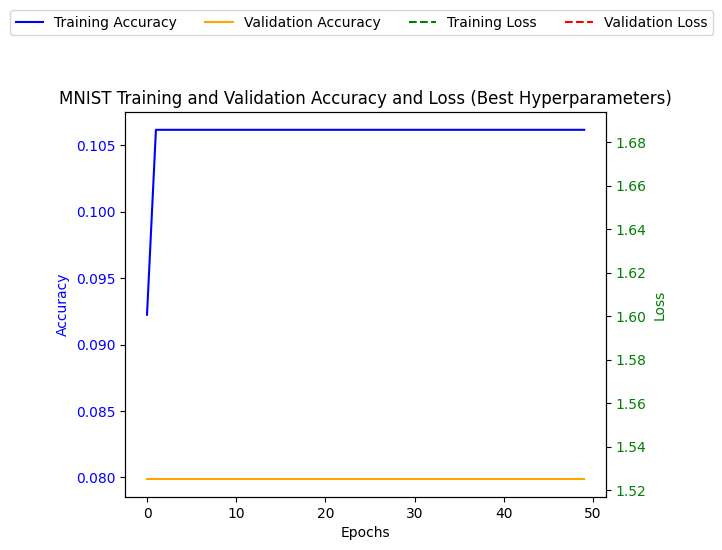
\includegraphics[width=0.8\linewidth]{failed_adam.png}
    \caption{Failed convergence due to the initial bias correction bug in the Adam optimizer implementation.}
    \label{fig:failed_adam}
\end{figure}

Correcting the initialization of `t` to 1 allowed the bias correction to operate correctly from the beginning of training. This modification was critical, especially in the early stages of training, and enabled the optimizer to update the weights accurately, leading to the successful training outcome shown in Figure \ref{fig:successful_adam}.

The second moment estimate's adaptive learning rate is instrumental in dealing with sparse gradients and non-stationary objectives, allowing the optimizer to adjust the learning rate for each parameter based on its gradient history. This feature is highlighted in our corrected implementation, where the network's convergence demonstrates the Adam optimizer's robustness to initial conditions and gradient variance.

In summary, our findings validate the literature on the effectiveness of the Adam optimizer. Its dynamic adjustment of learning rates coupled with momentum-based updates provides a strong foundation for training deep neural networks. While we observed significant benefits with default hyperparameter settings, we anticipate that a dedicated hyperparameter search could unlock further enhancements in the network's performance.


\section{Conclusions}
\label{sec:conclusions}
This study underscores the intricacies of manual neural network construction and the paramount importance of hyperparameter optimization. Momentum and adaptive learning rates have emerged as critical components for improving network training dynamics. While our scratch-built ANN provided valuable insights, it also revealed the challenges and complexities that high-level libraries like Keras abstract away. Future work could focus on refining the Adam implementation, exploring alternative optimization strategies, and scaling the network to tackle more complex tasks.

\section*{Acknowledgments}
I'd like to thank ChatGPT \cite{ChatGPT2023} for assistance with formatting, editing, and LaTeX support throughout this assignment.

\bibliography{aaai23}

\end{document}

